\chapter{Einleitung}
\label{cha:einleitung}

Das Internet of Things ist mittlerweile ein gut etabliertes Konzept, welches nicht nur den Einzug in das tägliche Leben vieler Menschen bewältigt hat, sondern auch in Großprojekten wie etwa beim Speditions- und Logistikunternehmen UPS [\cite{ups}] oder dem Gerätehersteller John Deere [\cite{johndeere}] Anwendung findet. Allerdings finden die Planung und Steuerung von Fertigungsprozessen bei konventionellen Fertigungsstraßen immer noch meist auf spezieller, proprietärer Hardware und vor Ort bei der Maschine statt. Um dies an moderne Gegebenheiten wie Heimarbeit oder Fernwartung anzupassen und um die Prozess-/Produktionsplanung und -steuerung zugänglicher zu machen, ist eine Modernisierung der Schnittstellen und Benutzeroberflächen nötig.

Das Institut Datenverarbeitung in der Konstruktion (DiK) beschäftigt sich unter anderem eingehend mit den Themen Industrie 4.0 und Industrial Internet of Things (IIoT) und hat eine Vielzahl von Kooperationen mit nationalen und internationalen Partnern. In der Forschungseinrichtung wird eine moderne und für die Industrie repräsentative Fertigungsstraße (abgebildet in Grafik \ref{fig:dikAnlage}) eingesetzt, um das Potenzial von Industrie 4.0 und IIoT Applikationen zu analysieren. Als didaktische Plattform dient hierfür die Webseite Digital Twin Academy (\href{https://digitaltwinacademy.de/}{digitaltwinacademy.de}).
%
\begin{figure}[htbp]
	\centering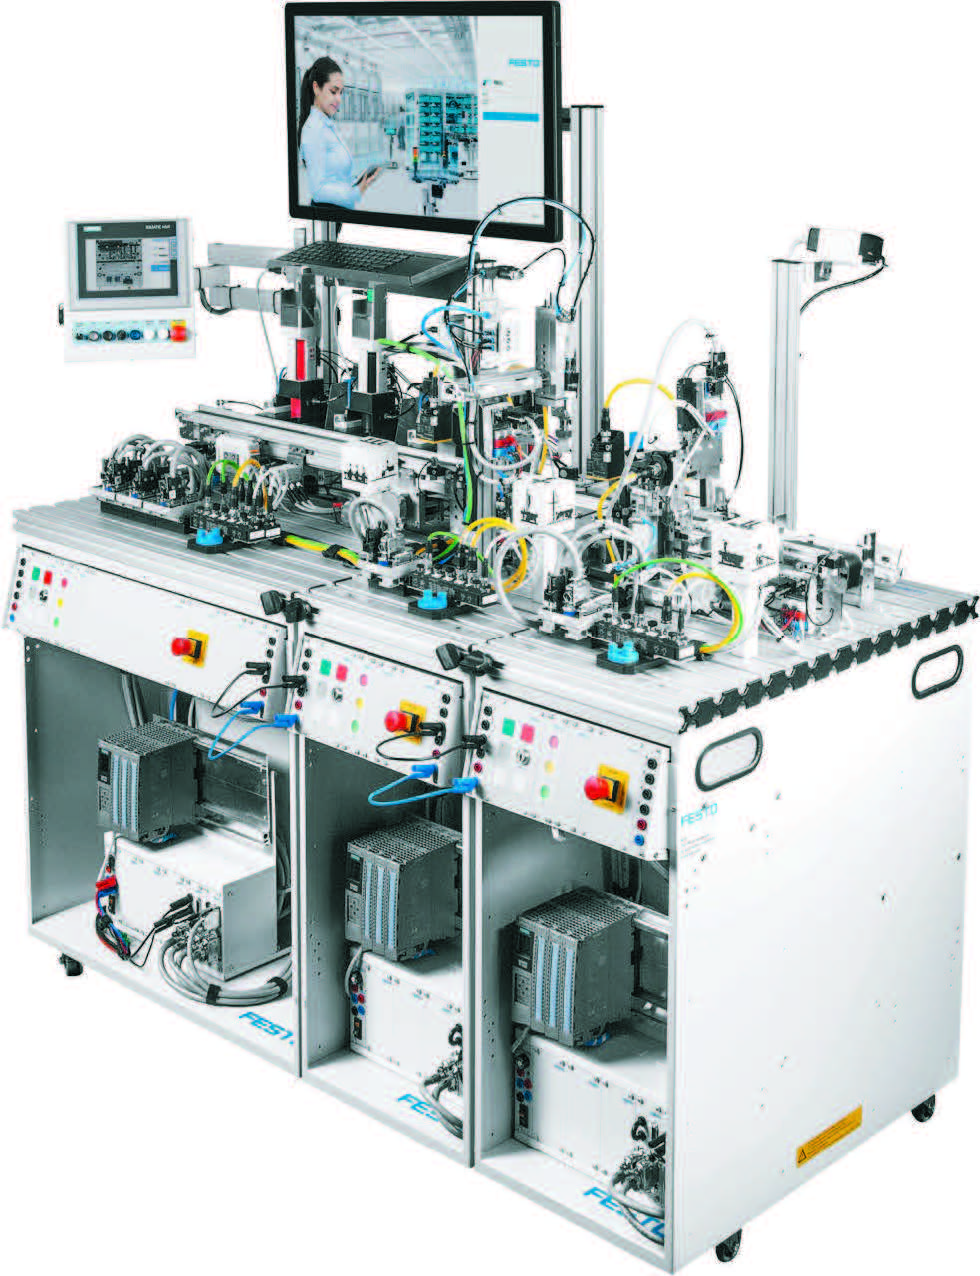
\includegraphics[width=0.5\textwidth]{images/01/DiK_Anlage.jpg}
    \caption{Festo MPS System 403-1 am DiK}
    \label{fig:dikAnlage}
\end{figure}

\subimport*{}{1_Motivation}
\subimport*{}{2_Zielsetzung}
\subimport*{}{3_Aufbau}
